\label{mathModel}
% TODO explain that int_x int_y h(x,y) dx dy = 1 
\section{What is an image?}

An image is a two dimensional signal $f(x,y)$ that takes the position of a point on a plan as argument and returns the luminance intensity at that point. If the image is gray-scaled, the output is a scalar:
\begin{eqnarray}
f:\Omega \rightarrow \mathbb{R}: (x,y) \mapsto f(x,y),
\end{eqnarray}
where $\Omega \rightarrow \mathbb{R}^2$. If we have a coloured image, we adopt a RGB (Red-Green-Blue) representation and the output will be 3-dimensional (one dimension per primitive colour):
\begin{eqnarray}
f:\Omega \rightarrow \mathbb{R}^3 : (x,y) \mapsto f(x,y).
\end{eqnarray}
Along this report, we will only consider gray-scaled images but we can easily generalize the problem to coloured images. $f$ is a continuous signal. But to be able to manipulate an image, we will often have to discretize this signal. The discretized signal is then of the form $f(m,n)$, where $m=1...M$ and $n=1...N$ with $M,N \in \mathbb{N}_0$. The signal can then be represented by a matrix $F$ (3 matrices for coloured images). An element  of this matrix is called a pixel. The values of $f(m,n)$ are often represented by words of $8$ bits so $f(m,n)$ can take $256$ different values: $f(m,n) \in \left[0...255\right]$.

\section{What is blurring?}

Blurring is the operation of mixing the spatial information of an image. In this section, we will try to give an accurate description of an continuous model and a discrete model of blurring.

\subsection{Continuous model}

Let $\mathcal{H}$ denote the operator of blurring. If $f(x,y)$ is the original image and $g(x,y)$ the blurred version of it, then we can represent the operation of blurring by the system shown on figure (???) or by the following equation:
\begin{equation}
g(x,y) = \mathcal{H}\left\lbrace f(x,y) \right\rbrace.
\end{equation}

\begin{figure}
\begin{center}
\begin{tikzpicture}[every text node part/.style={align=center}, every node/.style={scale=0.7},scale=0.7]

\draw(3,0)--(7,0)--(7,3)--(3,3)--(3,0);

\draw(5,1.5)node{blur \\ $\mathcal{H}$};

\draw[->](0,1.5)--(3,1.5);
\draw[->](7,1.5)--(10,1.5);

\draw(0,1.5)node[above]{f(x,y)};
\draw(10,1.5)node[above]{g(x,y)};

\end{tikzpicture}
\end{center}
\caption{System representation of blurring}
\label{system}
\end{figure}

We suppose the blurring operator to be linear. This assumption will be verified in the specific situations we have chosen (train and camera). Mathematically, we write:
\begin{equation}
\mathcal{H}\left\lbrace \alpha f_1(x,y) + \beta f_2(x,y) \right\rbrace =  \alpha \mathcal{H}\left\lbrace f_1(x,y)\right\rbrace + \beta \mathcal{H}\left\lbrace f_2(x,y)\right\rbrace,
\end{equation}
for $\alpha, \beta \in \mathbb{R}$.
Secondly, we may assume the operator is shift-invariant: when the input signal is shifted, the output signal is shifted by the same amount. This implies that the blurring system responds identically, no matter where on the plan the input is applied, which seems intuitively correct for images where all the objects of the scene are approximatively on the same vertical plane (this is an assumption we will make in the specific situations, cfr. infra). Mathematically:

if $\mathcal{H}\left\lbrace f(x,y) \right\rbrace = g(x,y)$, then $\mathcal{H}\left\lbrace f(x-x_0,y-y_0) \right\rbrace = g(x-x_0,y-y_0)$.

The input signal can be represented by a weighted superposition of shifted impulses \cite{haykin2007signals}. Because of the linearity of the system, the output is a weighted superposition of the responses of the system to each shifted impulse. The system is also shift-invariant so the system's response to a shifted impulse is a shifted version of the system's response to an impulse. Hence, the output is given by a weighted superposition of shifted impulse responses. This weighted superposition is called $\emph{convolution}$. So, if $f(x,y)$ is the input, $h(x,y)=\mathcal{H}\left\lbrace \delta(x,y) \right\rbrace$ ($\delta(x,y)$ is an impulse) is the system's impulse response and $g(x,y)$ is the output, then we write:
\begin{eqnarray}
g(x,y) &=& \mathcal{H}\left\lbrace f(x,y) \right\rbrace \\
g(x,y) &=& h(x,y) \ast f(x,y),
\end{eqnarray}
where $\ast$ is the convolution symbol. So blurring is spreading the value of a pixel by a certain way which is determined by $h$. That's why we call $h$ also the Point Spread Function (PSF).

When we take a picture, the image that we get is usually affected by additive noise. Additive means that the noise does not depend on the input signal. If $e(x,y)$ denotes the additive noise, we can represent the system by the scheme  given in figure $(\ref{systemnoise})$ or by the following equation:
\begin{eqnarray}
g(x,y) &=& \mathcal{H}\left\lbrace f(x,y) \right\rbrace + e(x,y) \\
 &=& f(x,y) \ast h(x,y) + e(x,y).
\label{generaleq}
\end{eqnarray}
This noise represents measurement and round-off errors and also errors due to the model (convolution) we use to represent blurring.

\begin{figure}
\begin{center}
\begin{tikzpicture}[every text node part/.style={align=center}, every node/.style={scale=0.7},scale=0.7]

\draw(3,0)--(7,0)--(7,3)--(3,3)--(3,0);
\draw(5,1.5)node{blur \\ $\mathcal{H}$};

\draw(10.5,1.5)circle(0.5);
\draw(10.5,1.5)node{$+$};

\draw[->](0,1.5)--(3,1.5);
\draw[->](7,1.5)--(10,1.5);
\draw[->](10.5,5)--(10.5,2);
\draw[->](11,1.5)--(14,1.5);

\draw(0,1.5)node[above]{f(x,y)};
\draw(11,1.5)node[above]{g(x,y)};
\draw(10.5,5)node[right]{n(x,y)};

\end{tikzpicture}
\end{center}
\caption{System representation of blurring with noise}
\label{systemnoise}
\end{figure}


\subsection{Discrete model}

Like we said earlier, in the discrete model, the signals can be represented by matrices. The operation of $\mathcal{H}$ on $f$ can then be replaced by a matrix multiplication of $H \in \mathbb{R}^{M \times M}$ (the matrix associated with the operator $\mathcal{H}$) with $F \in \mathbb{N}^{M \times N}$ (the matrix associated with the input signal $f$). Equation $(\ref{generaleq})$ becomes:
\begin{equation}
G = HF + E,
\label{eqmatrix}
\end{equation}
where $E \in \mathbb{R}^{M \times N}$ is the matrix associated with the additive noise $e$. To handle this problem more easily, we would like to solve a linear system. That's why we are going to make a vector of a matrix representing an image. So if $F \in \mathbb{N}^{M \times N}$ is a matrix representing an image, then the corresponding vector $\emph{f} = vec(F) \in \mathbb{N}^{MN \times 1}$ is constructed by putting the columns of $F$ under each other. Watch out for the notation used: $f$ is a continuous signal, $F$ is the matrix associated with this signal and $\emph{f}$  is the vector corresponding to this matrix. Equation $(\ref{eqmatrix})$ becomes:
\begin{equation}
\emph{g} = \tilde{H}\emph{f} + \emph{e},
\label{eqvec}
\end{equation}
where $\tilde{H} \in \mathbb{R}^{mn \times mn}$ is the result of the following Kronecker product:
\begin{equation}
\tilde{H} = I_n \otimes H,
\end{equation}
with $I_N$ the identity matrix of dimension $N$. By equation $(\ref{eqvec})$, we clearly see that a pixel of the blurred image is a linear combination of pixels of the original image, plus some noise. In the following section, we will always take the matrix form of an image but the vector form can be easily get by the equations just above.

\section{What is deblurring?}

Deblurring is the inverse operation of blurring. So it consists in getting the image $F$ from the blurred image $G$. Let's take the model without noise:
\begin{equation}
\emph{g}=H\emph{f}.
\end{equation}
If the blurring matrix $H$ is known, deblurring is just solving a linear system and there a lot of different algorithms to do that. But in a real situation, we only have the blurred image $G$ and we don't know $H$. That's why we approximate $H$, knowing some information about how the image has been blurred. Finding this approximation is the subject of the following section. If we take the noise into account, the problem becomes ill-posed. We then apply the regularisation of Tikhonov:
%TODO Tikhonov

\section{Specific situations}

Like we said in the previous section, to approximate the blurring operator, we need some information on the reason why the image has been blurred. We have chosen two typical situations in which blur effect occur. The first one is a a picture that has been taken from a moving train wtih known or unknown speed. The second one is a picture depicted by a security camera. The goal is to deblur the part of the image where a subject is moving. We also dispose of several statistical images without the subject.

\subsection{Train}

First we need to make some assumptions about the circumstances to get an idea of what $H$ should look like. We assume that the picture has been taken with the camera parallel to the train (hyp. 1). This means that the blur effect will only appear horizontally on the picture. We also assume that the speed of the train is constant during the short period of time when the picture is taken (hyp. 2). This allows us to suppose the blurring operator to be linear: every pixel is modified in the same way. If the speed isn't constant, the parts of the image where the camera is going faster, are influenced by more pixels then the parts where the camera is going slower. The operation is not linear anymore and we won't take this case into account. We will first treat the case where the speed of the train is known and then when it is unknown. Finally we suppose the subjects on the picture to be in the same vertical plane (hyp. 3). So every subject lies approximatively on the same distance away from the camera. This also means that blurring will approximatively have the same effect everywhere on the image. If this was not the case, the blur effect would be more visible on subjects near the camera.

Based on all those assumptions, we can now build an approximative form for the blurring matrix $H$. So we have to answer to the following question: ``How is a pixel of $G$ constructed based on the pixels of $F$?''. Through hypothesis 2, we know that only the pixels belonging to the same row as the pixel of $G$ that we are studying, will influence that pixel. If the train is travelling to the left (respectively to the right), a certain number of pixels on the right (respectively left) of that pixel will influence it. Let's denote this number of pixels by $k$. By linearity, we can say that the blurred image is a weighted superposition of shifted versions of the original image. If $D$ is a matrix representing the operator that shifts the image by one pixel horizontally, we can define the blurring matrix $H$ as:
\begin{equation}
H=\sum\limits_{i=0}^{k} c_i D^{i}.
\label{eqHtrain}
\end{equation}

Now we still have to determine $k$ and the factors $c_i \in \mathbb{R}$ based on the assumptions we made. Let's begin by $k$. If the speed is unknown, we cannot find an analytical representation for $k$. This case will be treated in later chapters. So for now, we suppose the speed of the train known and denote it by $v$. Intuitively, we expect $k$ to be increasing when the speed or the opening time also do. On the opposite, $k$ should decrease when the average distance goes up. We already mentioned that before. If $\phi$ is the opening angle of the camera and $\eta$ is the average distance from the camera to the scene, we can represent the situation by figure (??). The width $W$ of the scene is then obtained by: 
\begin{equation}
W = 2 \eta \tan\left(\frac{\phi}{2}\right).
\end{equation}
A row of the matrix associated to the image ($F$) represents then a real line of the image of length $W$. If $F$ has $N$ columns, the width of one pixel $W_e$ is
\begin{eqnarray}
W_e &=& \frac{W}{N} \\
&=& \frac{2 \eta }{N}\tan\left(\frac{\phi}{2}\right).
\end{eqnarray}
We now want to know the time it takes to a real segment of length $W_e$ to be represented by the next pixel. We denote this time by $\Delta t_e$ and we get:
\begin{eqnarray}
\Delta t_e &=&\frac{W_e}{v}\\
&=& \frac{2 \eta }{Nv}\tan\left(\frac{\phi}{2}\right).
\end{eqnarray}
Finally, we compute $k$ knowing that it is the number of times $\Delta t_e$ can be put in the opening time $\Delta t$ of the camera:
\begin{eqnarray}
k &=& \frac{\Delta t}{\Delta t _e} \\
&=& \dfrac{Nv\Delta t}{2 \ eta \tan\left(\frac{\phi}{2}\right)}.
\end{eqnarray}

From this equation, we can verify our expectations: $k$ is proportional to $v$ and $\Delta t$, and inversely proportional to $eta$.

\begin{figure}
\begin{center}
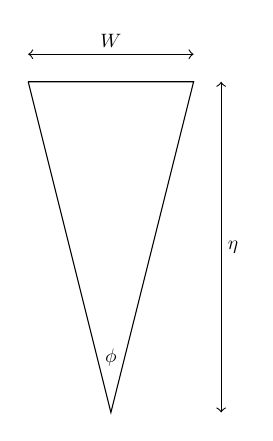
\begin{tikzpicture}[every text node part/.style={align=center}, every node/.style={scale=0.7},scale=0.7]

\draw(0,0)--(3,0)--(1.5,-6)--(0,0);
\draw[<->](3.5,0)--(3.5,-6);
\draw[<->](0,0.5)--(3,0.5);

\draw(1.5,0.5)node[above]{$W$};
\draw(3.5,-3)node[right]{$\eta$};
\draw(1.5,-5)node{$\phi$};

\end{tikzpicture}
\end{center}
\caption{Representation of the situation when the picture is taken.}
\label{situation}
\end{figure}

Now what about the coefficients $c_i$? Let's suppose the train is travelling to the right, so a pixel $G(m,n)$ is a weighted sum of the $k$ pixels to the left of the corresponding pixel $F(m,n)$ (plus itself). As the speed of the train is constant, every weight should be equal. Pixels of $G$ also have a range from $0$ to $255$ so the weighted sum must not exceed the maximum. That's why we have $c_i=\frac{1}{k+1}$.

The last thing we need to determine in  equation $(\ref{eqHtrain})$ is the matrix $D$. A first version of it for a $3 \times 3$ image could be (we are still considering the train is moving to the right):
$$
\begin{pmatrix}
a & b & c \\
c & d & e \\
f & g & h \\
\end{pmatrix}
\begin{pmatrix}
0 & 1 & 0 \\
0 & 0 & 1 \\
0 & 0 & 0
\end{pmatrix}
=
\begin{pmatrix}
0 & a & b \\
0 & c & d \\
0 & f & g \\
\end{pmatrix}.
$$
Suppose we model the blurring of this $3 \times 3$ matrix $F$ with $k=1$ (we neglect the noise effect). We then have $G(i,3) = \frac{1}{2} F(i,2) + \frac{1}{2} F(i,3)~i=1,2,3$, just like we expected. It also works for the second column. But for the first column, we get: $G(i,1) = \frac{1}{2} F(i,1)~i=1,2,3$ so it only makes the left border of the original image darker (as 0 is black and 255 is white). If we took a bigger $k$, we would observe this for all the columns for which $n \leq k$ as they need some information out of the image. Actually, with this matrix $D$, we considered that everything that is beyond the scope of the image is black, and that is of course a bad approximation. So to get a better information about what is beyond the left edge of the image, we could approximate it by extrapolation. A simple example is the polynomial extrapolation of order 0. This consists in putting the first column $k$ times on the left of the image. Using the same example, we get:
$$
\begin{pmatrix}
a & b & c \\
c & d & e \\
f & g & h \\
\end{pmatrix}
\begin{pmatrix}
1 & 1 & 0 \\
0 & 0 & 1 \\
0 & 0 & 0
\end{pmatrix}
=
\begin{pmatrix}
a & a & b \\
c & c & d \\
f & f & g \\
\end{pmatrix}.
$$
Now we have : $G(i,1) = F(i,1)~i=1,2,3$, which is a bit better than the previous model. If we take a higher order of extrapolation, we get a better approximation of the real blurring effect.

%TODO pas compris le truc avec le C_1-j pour l'extrapolation d'ordre 1

Another way to treat those ``edge problems'' is by modelling the blur effect on a smaller image. If we apply our model on the image defined by $F_{small} = F(m,n)$ for $m>k$, then we have all the ``missing information'' and we don't need to extrapalte anymore.


\subsection{Security camera}

Our next situation is a fixed camera taking a sample of pictures with everytime the same scene but sometimes disturbed by a person walking around. The goal is to deblur the part of the image where a person is walking. There are three differences compared to the situation with the train. Firstly, only a part of the image is blurred, so deblurring will also be only applied on that part. Moreover, if the person is not too close to the edges of the image, we don't have any ``edge problems'' anymore. And finally, the person could walk in any direction so we don't have a perfect horizontal blur effect anymore.

Now how can we detect a walking person on an image? If we have a high number of statistical images, we can build a background-image that contains the average value of each pixel. If we take the difference between the blurred image and this image, we get an image that contains very small values (near to zero) for the regions where the person is not present and bigger values for the regions that we call the foreground. Next we extract the foreground and we deblur this new image.
